\chapter{Introduction}\label{sec:introduction}

Statewide travel forecasting models have become an essential tool for transportation planners over the past two decades. They are used in a variety of planning and programming activities at the state and regional level to evaluate policy and investment options. They also provide information to metropolitan models, and many agencies use their statewide modeling program as the impetus for developing best practices in travel modeling at all levels of geography within the state. However, many of these advances have occurred only recently. The number of operational statewide models increased from 40 percent a decade ago \citep{horowitz06} to 65 percent today, with an additional nine percent having a model under development. They are used to formulate plans and policies, evaluate and prioritize projects and programs, and to assess the economic and social impacts of major transportation investments. Typical studies conducted with them include bypasses around congested areas and assessment of improved commuter rail lines on auto dependency before costly projects are constructed. Depending on analysis needs, such models have been coupled with environmental impact models, economic models, land use models or fiscal impact models. However, transportation remains the dominant focus of all statewide models in operation today.

Megaregional modeling is still in its infancy, despite the revised interest in this level of analysis in the U.S. \citep{amekudzi07, florida08}. Except for the Chesapeake Bay Megaregional Model \citep{moeckel15b}, described in \S\ref{sec:chesapeake-bay-megaregion-model} (page \pageref{sec:chesapeake-bay-megaregion-model}) as a case study, no megaregion in the U.S. has an operational transportation model as of 2016. Given the growing interests in megaregional analyses and the similarity to statewide models, requirements and recommendations for megaregional models are discussed in this report as well.

The purpose of this synthesis report is to document the current state of statewide and megaregional modeling, to describe common model applications, to document data requirements, to identify limitations in current model design and to provide ideas and trends for the future development of such models.

\section{Background}

Stakeholders in statewide and megaregion models, including state transportation agencies, regional planning agencies, the Federal Highway Administration (FHWA) and the University Transportation Centers, have a wealth of experience on technical advances, as well as organizational challenges such as implementation sequencing, funding mechanisms, staffing and data sources. This Synthesis Report provides a snapshot of current models, including the methods and practices that states and other agencies have employed to develop effective and affordable large area models.

Currently, 30 states have operational statewide models with varying levels of maturity and complexity. In addition, several multi-state and megaregional models have been created for various special purposes. FHWA is conducting exploratory research on national person and freight travel models.

This Synthesis Report broadly documents how the state of the practice in national, megaregional, and statewide travel demand modeling has continued to evolve. It addresses:
\begin{itemize}
\item The reasons for creating statewide and megaregional models, and how these models have responded to SHRP2 and performance measures in federal transportation bills.
\item National, multi-state, megaregional and statewide travel demand models across the nation, addressing both passenger and freight, comparing the models, focusing not just on the current state of the model but also the past and projected development path followed by the agency.
\item The hierarchical nature of statewide versus regional models, what model type is best for different analyses, and the pros and cons of using common data assumptions and sources.
\item The data used in large area models, their availability, and technical and other challenges in using new and emerging passive data sources as well as data-driven forecasting techniques
\item Existing and emerging applications of large area models including high-speed and intercity rail projects, multi-state corridor projects, tolling analysis/funding shortfalls, project prioritization and design, freight planning, economic analysis, and traffic forecasting needs external to metropolitan planning organization (MPO) areas.
\item Specific examples of advanced methods used in the large area travel demand models that better reflect congestion and reliability outcomes. These include integrated land use models, population synthesis, tour-based models, economic models dependent upon large-area TDMs, and time-sensitive network techniques such as dynamic traffic assignment.
\item   Emerging trends for simplified and strategic models for rapid response to policy issues, including shorter run times.
\item Institutional constraints on data consistency
\end{itemize}

The information used to prepare this report included literature reviews, documentation from known existing models, and a survey of the voting members of the AASHTO Standing Committee on Planning and other groups.

\section{Study approach}

Statewide modeling is a diverse field of practice. Model frameworks reach from rather simple aggregate three-step models to quite sophisticated activity-based microscopic modeling approaches. Several methods were undertaken to gather information about the variety of statewide modeling approaches used in the USA. These included a formal survey of planners in all 50 states, an informal survey of leading practitioners, and detailed review of several case studies. A literature review complemented these efforts. While published materials on statewide modeling are somewhat limited, additional literature on travel demand modeling with a focus on long-distance travel was added. Also, some background on freight and land use modeling was collected during the study. The surveys are described in the following sections, while the case studies are profiled in Chapter \ref{sec:case-studies}.

\subsection{Survey on statewide modeling practices}

A detailed survey of statewide modeling practices was sent to voting members of the AASHTO Standing Committee on Planning. It was designed as an online survey that could be filled out anytime and anywhere at the respondent's pace. The software further allowed respondents to fill in part of the survey, save it and resume later. This functionality also enabled respondents to fill in parts of the survey and hand over the partly completed survey to a colleague who may be an expert in a certain subsection of the survey.

The survey attempted to balance the desire for obtaining detailed information with the burden of completing it. An initial version with 22 questions was examined by the review panel of this Synthesis Report and improved based on the panel's feedback. A pretest was conducted with the states of Ohio and Oregon in early March 2016. It confirmed the functionality of the survey software, helped to refine phrasing of selected questions and expanded the survey slightly. Long-distance travel was added as a separate topic to the survey based on the pre-test feedback. The final version with 27 questions was longer than initially anticipated but necessary for collecting sufficient detail on statewide modeling. The time needed to fill out the survey was reported by the pre-testers to be 30 to 45 minutes. However, some respondents spent less time, especially from states that do not operate statewide models. Others spent more time, particularly those that put in extra effort to research answers for some of the questions. The survey design was finalized two weeks later. A copy of the final survey form can be found in Appendix \ref{sec:appendix-a-survey-questionnaire}.

The invitation to participate in the survey was sent to the Members of the AASHTO Standing Committee on Planning (SCOP) by email on March 21st, 2016. Initially, a response was requested by April 8th, though this deadline was postponed after reminder emails were sent to those states that did not fill out the survey right away. Forty-six states responded to the survey between March 22nd and May 30th.

The distribution of states with and without models is shown in Figure \ref{fig:states-with-operational-models}. Not surprisingly, many states without models are predominately rural with little congestion. However, such states often face several other equally important issues, such as allocation of limited funding, that statewide models can inform. At the other end of the spectrum, New York does not operate a statewide model despite being the seventh densest state in the U.S. However, New York's density is heavily driven by the New York City Metropolitan Area, which operates its own (urban) transportation model.

\begin{figure}
\centering
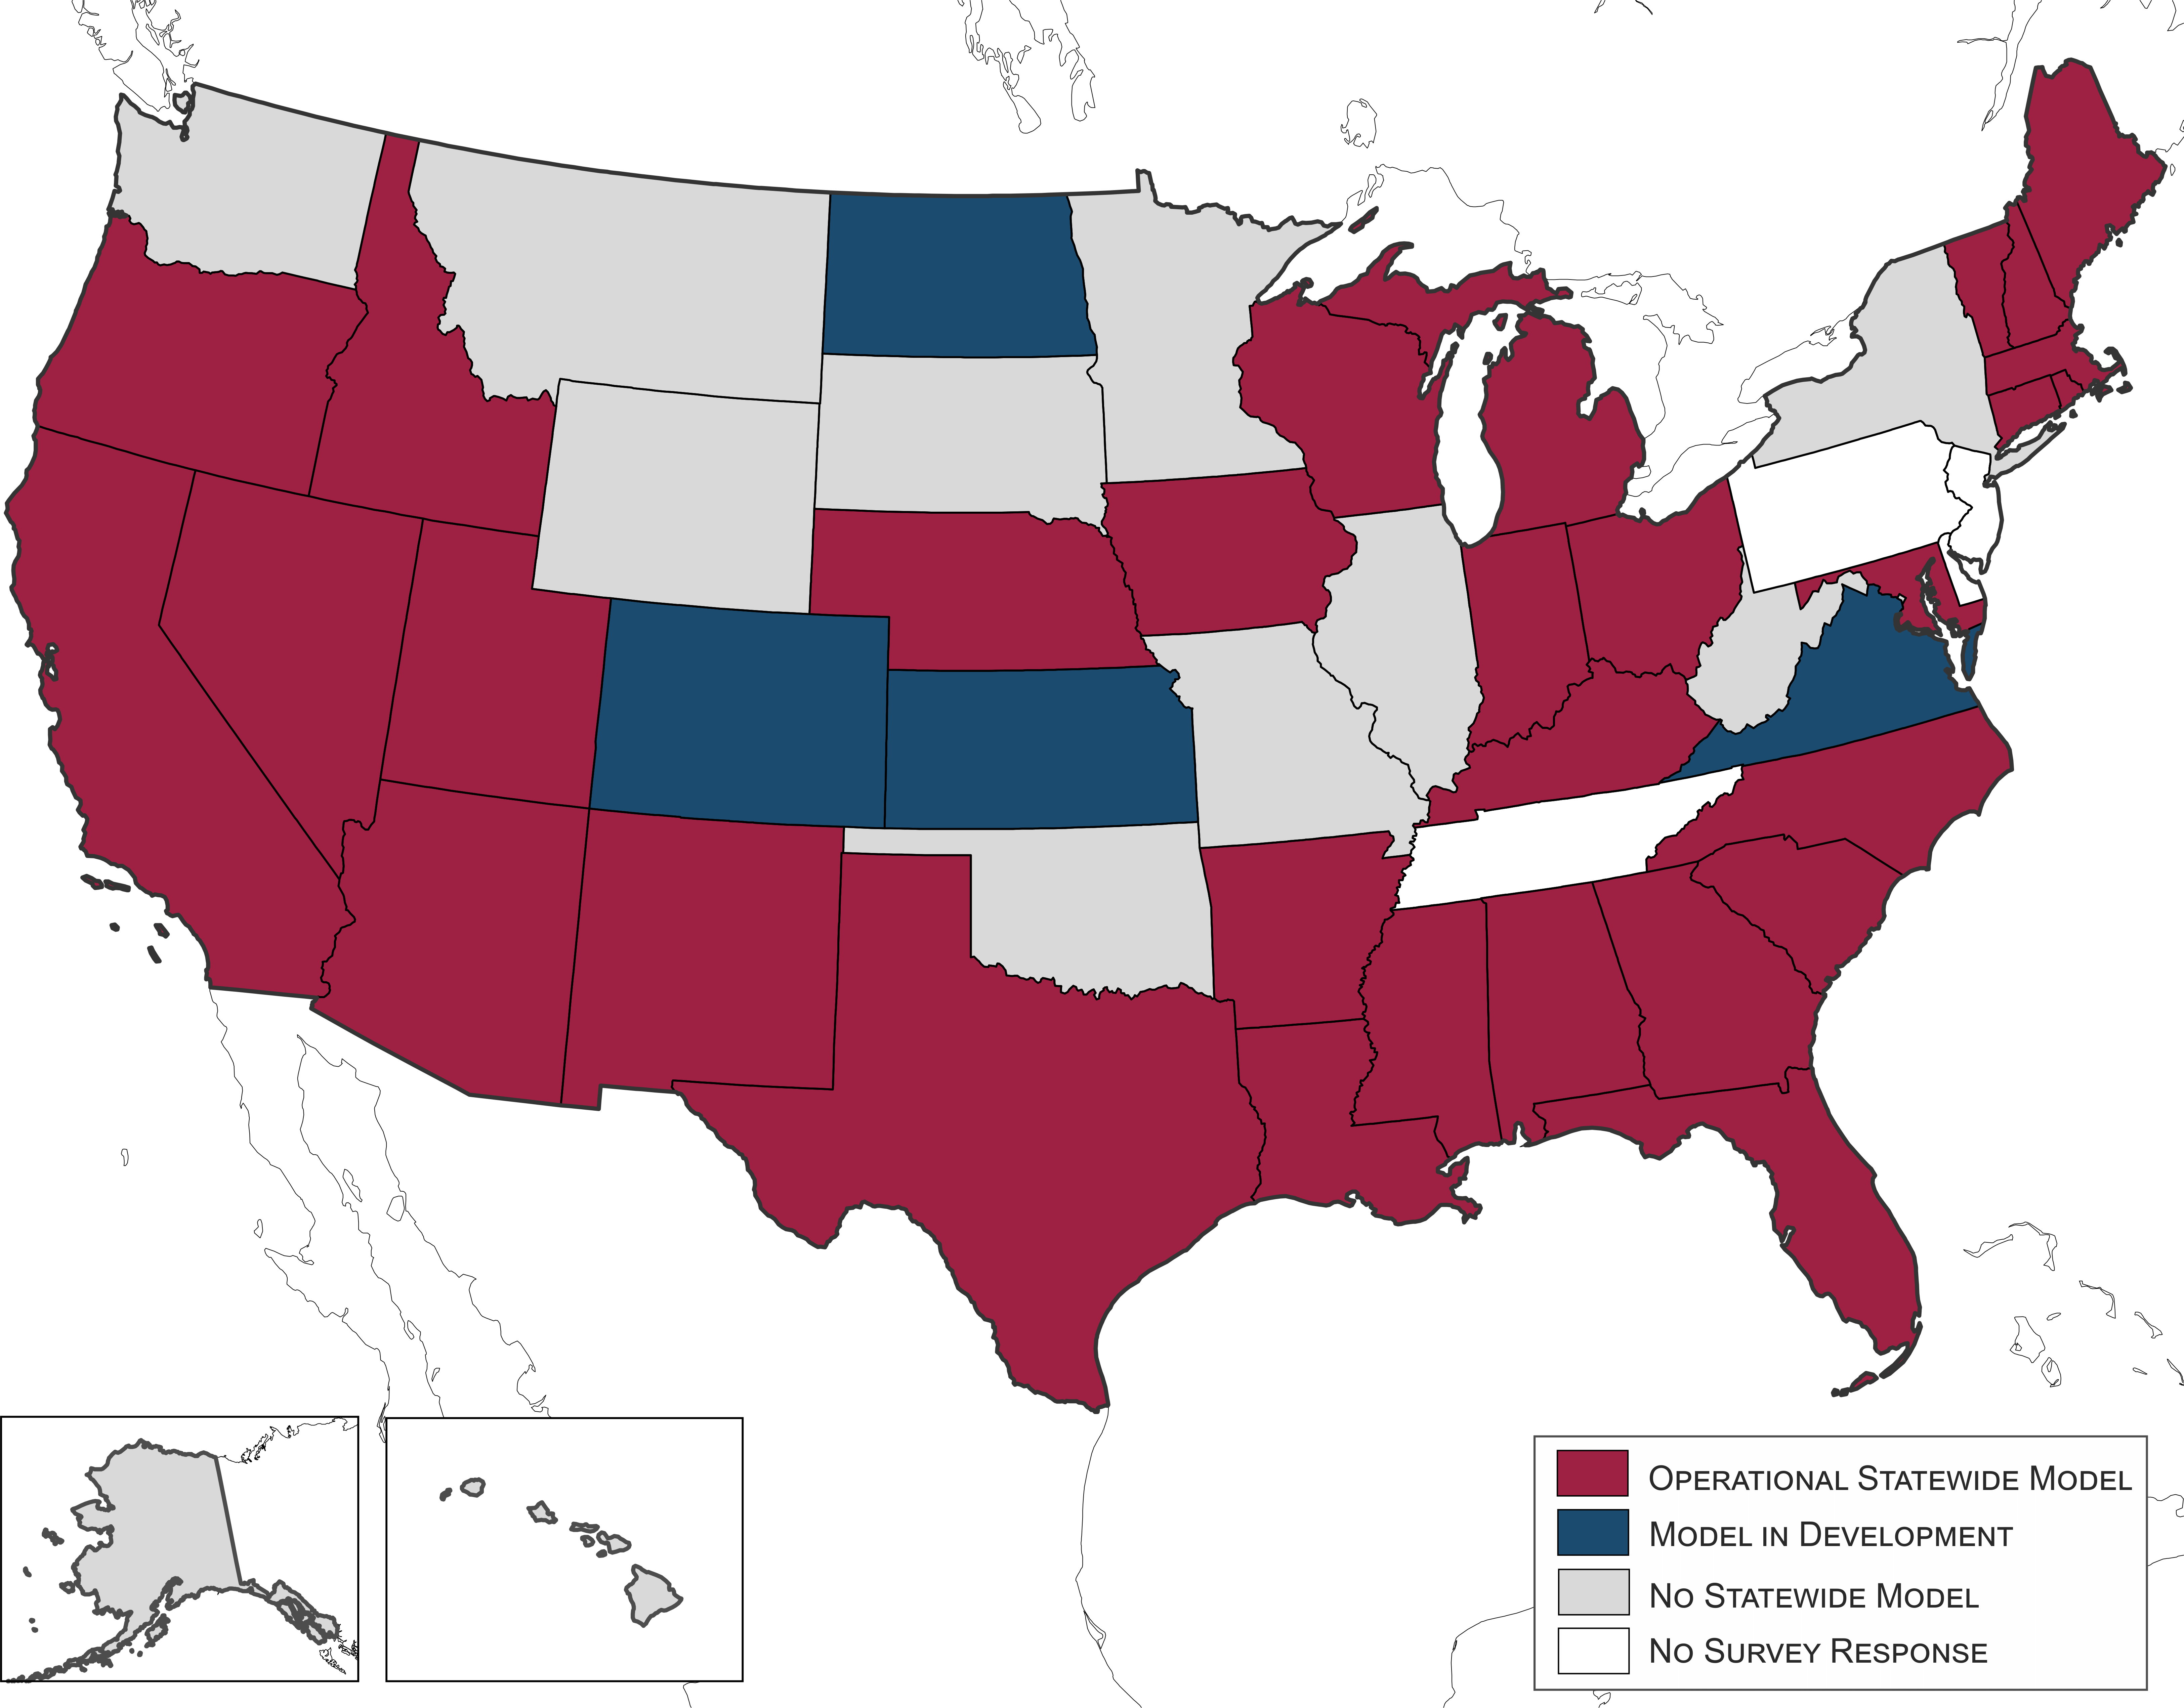
\includegraphics[width=6in]{graphics/01-states-with-operational-models}
\caption{States with operational statewide models}
\label{fig:states-with-operational-models}
\end{figure}

The number of states that responded are summarized in Table \ref{tab:states-conducting}. The response rate was 92 percent. Of the states that responded, 74 percent either operate or are developing a statewide model.

\begin{table}  % 1
\centering
\caption{States conducting statewide modeling}
\label{tab:states-conducting}
\begin{tabular}{lcl}
\hline
Response category & Number of states & Percent \\
\hline
Invited to participate in survey & 50 & 100 \\
Responded & 46 & 92 (of all U.S. states) \\
\hline
Operate a statewide model & 30 & 66 (of states that responded) \\
Developing a statewide model & 4 & 9 (of states that responded) \\
All others & 12 & 12 (of states that responded) \\
\hline
\end{tabular}
\end{table}

The survey also revealed that many states have developed add-on models that support the transportation model. Fifteen states operate separate long-distance travel models, 28 states have some form of freight model, nine states model environmental impacts, and two states formally model land use changes. The survey results are presented in detail in Chapter \ref{sec:survey-existing-practice}.

\subsection{TRB statewide modeling subcommittee survey}

The formal survey was supplemented by an informal survey of members of TRB's subcommittee on statewide modeling, conducted during May 2016. The members of the subcommittee are leaders in the development and application of statewide models, with members from state and federal government, academics, and consultants engaged in this type of work. The following open-ended questions were posed to the subcommittee members and friends:
\begin{enumerate}
\item What are the most important analytical issues that you have recently used statewide models to evaluate? How suitable were the tools and data for the task? Did you encounter any noteworthy issues or challenges? 
\item What emerging trends or issues have decision-makers asked you for help evaluating, but for which your model was not up to the task for? In the same vein, what new questions do you expect to be hit with in the near future?
\item What data, methodological, and institutional barriers are holding statewide modeling back?
\end{enumerate}

Three email replies were received, and eight additional interviews were conducted by telephone or during the TRB Innovations in Travel Modeling conference in early May 2016. The small number of responses precluded tabulation, although each conveyed substantial information. Their insight was illuminating, and certain themes and issues came to light. The analytical issues facing statewide modelers (Question 1) varied widely, resulting in the extensive list shown in The evaluation of projects with multi-jurisdictional impacts was the most frequently cited, followed closely by statewide transportation plan development and prioritization.

Most of the respondents felt that their current models were adequate, suggesting the diversity of modeling approaches described in Chapter \ref{sec:survey-existing-practice} can usually address the specific needs of each client. They likely feel less inclined to update their modeling platforms to more advanced models, given the adequacy of existing models for their needs. The considerable momentum towards activity-based models in congested urban areas has only rarely carried over to statewide modeling, in part because most states appear to lack the resources required to do so.

\begin{table}  % 2
\centering
\caption{Frequently cited issues studied with statewide models}
\label{tab:frequent-issues}
\begin{tabular}{|l|}
\hline
Evaluation of projects with multi-jurisdictional impacts \\
Statewide transportation plan development \\
Statewide project ranking and prioritization \\
High-speed rail feasibility studies \\
Major corridor studies \\
Impact of economic downturn on travel patterns \\
Modeling travel patterns outside of MPO modeled areas \\
Understanding truck flows and origin-destination patterns \\
Network continuity and resiliency analyses \\
Assessment of infrastructure degradation and disruptions \\
Assessing potential for truck-rail diversion \\
Provide inputs to economic impact or environmental models \\
Likely increases in VMT attributable to lower fuel prices \\
Analysis of weight-miles taxes and other demand-based revenues \\
Disinvestment (abandoning or curtailing infrastructure maintenance) \\
\hline
\end{tabular}
\end{table}

The largest reported challenges included:

\begin{itemize}
\item
The lack of precision in the model for detailed corridor studies was often cited. Stated differently, the same levels of spatial, temporal, and behavioral resolution found in urban models were desired at the statewide level. However, stretching an urban model to cover an entire state is impractical and too costly to build and maintain in most cases.
\item 
A lack of data on visitors and their travel patterns was often cited as a significant limitation for some project or corridor studies.
\item 
Too much time went into the development of some models, and too little into the user interface and visualization of model results. This made the models more difficult to use than their urban cousins, although it was acknowledged that many of the latter suffer from the same limitations.
\item 
Coding networks, especially for future years, is very labor-intensive and time-consuming. This was particularly an issue when analysts were asked to include all the capacity or operational improvements across a larger state.
\end{itemize}

The three most common emerging issues identified (Question 2) revolved around the expected benefits of big data, development of multimodal project evaluation or cost-benefit analysis processes, and the likely effect of autonomous and connected vehicles. It is hoped that big data, in the form of passively collected origin-destination patterns and travel times from cellular devices, will fill data gaps at an affordable price point, particularly for freight and commercial vehicle flows. Some viewed this as adding value to traditional revealed and stated preference surveys, while others felt that it opens the door to new modeling approaches.

Some states use a formal economic impact framework, such as TREDIS, in project evaluation, while others are still working on potential approaches. A recent survey of such models by \cite{holian16}, which suggests the use of ad hoc methods until better solutions become available, was also cited.

Modeling the effects of autonomous and connected vehicles is a hot topic at this writing, for which the respondents felt unprepared to address. How to formulate forecasts for a society where such vehicles dominate, and travel choices change in response to them, remain open questions. \cite{issac16} summarizes the likely policy impacts, as well as describing a range of different futures, depending on how society, laws, markets, and governments respond to this new mode of transportation. Beyond her work, however, there appears to be little to guide planners seeking to understand the likely impacts of autonomous vehicles, which respondents expect to be profound.

The largest challenges (Question 3) cited included the difficulty in attracting and retaining well-qualified staff, sporadic or uneven funding for statewide models, the difficulty of integrating or reconciling them with urban models, and the burden of obtaining information about regional or national travel affecting their state. All but one of the respondents felt that the staffing issue was the biggest challenge associated with statewide modeling. Most modelers are classified in pay grades too low to attract well-qualified applicants, forcing agencies to rely upon consultants, contract employees, or sometimes partnerships with MPOs, to gain access to the talent required to build and use such models.

The remaining challenges were cited only a few times, so perhaps less easy to characterize as broad issues. Inadequate funding for travel forecasting is often cited, but is not a problem unique to statewide modeling. The need for better integration of statewide models is a compelling issue that is described further in \S\ref{sec:urban-statewide-integration}. Recent federal data and modeling initiatives that can provide a compelling solution for statewide models are discussed further in \S\ref{sec:national-model-integration}.

\section{Megaregions}

The purpose of this Synthesis Report is to review both statewide and megaregional models. The two are similar in concept, both covering larger regions than urban travel demand models, often with a special focus on long-distance travel and freight flows. In some cases, statewide models and megaregional models may cover a very similar study area. Florida and Arizona are examples where much of the statewide modeling region is often considered one megaregion at the same time. The Texas statewide model covers a region even larger than the Texas Triangle megaregion (Houston-San Antonio-Dallas/Fort Worth).

On the other hand, there are two subtle yet significant differences between statewide and megaregional models, making it worthwhile to explore them separately. First, megaregions commonly ignore jurisdictional boundaries. Even the Florida and Arizona megaregions --- whose extent resembles their respective state boundaries --- do not follow jurisdictional delineations exactly. Some megaregions, such as the Northwestern region from Portland, Oregon to Vancouver, British Columbia or the Midwest megaregion around Chicago and Detroit, even reach across country boundaries into Canada. A megaregional perspective adds the potential to include all parts that functionally belong to a megaregion irrespective of administrative boundaries, yet it also poses the challenge of including stakeholders from different jurisdictions. The second difference between megaregional and statewide models is that the former tend to include fewer rural area and focus much more on the urban cores and their suburbs. Most megaregions focus on large metropolitan areas that are linked together economically or culturally, and rural parts are commonly are left out as the hinterland. Statewide models, in contrast, always cover at least the entire state area, and thereby, include rural and urban areas regardless of economic or cultural linkages.

\subsection{Definition of megaregions}

Megaregions across the Unites States have been analyzed for decades. The Boston-Washington corridor, the Chicago Metropolitan Region, and the Los Angeles Basin are prime examples of frequently studied megaregions \citep{florida08}. In Europe, one early megaregional concept, the Blue Banana, covers an arc stretching from Manchester in Northern England to Milan in Northern Italy. The Blue Banana was later rejected as being too simplistic (as it also covered the highly rural Alps). The European Grape was proposed as an alternative \citep{kunzmann01}, where every single grape abstracted a different European megaregion.

Formal megaregional arrangements are rare, even though political borders do not confine regional interactions and associated impacts. One notable quasi-megaregional agreement in the U.S. is the I-95 Corridor Coalition, a group of transportation agencies and toll authorities along the U.S. East Coast from Maine to Florida. However, being a volunteer and consensus-driven organization the Coalition is limited to actions that support the interests of all players involved. Similarly, the I-10 Coalition including the four states Arizona, California, New Mexico, Texas focuses on facilitating goods movements across this corridor. The Coalition focuses on a very specific topic, namely east-west freight flows of trucks. The Arizona Department of Transportation Director John Halikowski summarized the purpose as ``Someday we want the I-10 Corridor to be filled with truck platoons and connected vehicles, weigh-in-motion sensors and automated truck parking lots'' \citep{adot16}. Megaregional organizations with executive power do not exist in the U.S. to date.

On the other hand, megaregions comprise the economic engine of the U.S., are forecasted to contain half the nation's population growth, and perhaps up to two-thirds of its economic growth by 2050 \citep{amekudzi07}. Supporting the megaregions' economic competitiveness domestically and abroad is a key concern given increasing global competition and international trade. A primary justification for addressing policy issues at the megaregional scale as opposed to the metropolitan scale is that regional economic activities are increasingly linked. Economic shocks to one metropolitan area result in spillovers, both positive and negative, to adjacent metropolitan areas. Consequently, the resulting environmental and social impacts associated with such activities similarly spill across metropolitan areas. Furthermore, as pointed out by \cite{christaller33}, \cite{losch54}, and \cite{ross09b}, individual cities are part of larger systems that are linked by intercity trade hierarchies.

Megaregions are defined in multiple ways in the literature. Half a century ago, \cite{gottmann61} wrote a seminal book of the Northeastern Seaboard reaching from Washington to New York City, the largest urban conglomeration in the world at that time. An update was published by \citep{gottmann90}, in which the megaregion remained mostly defined by population densities. A more common approach, adopted by the U.S. Census Bureau and Bureau of Economic Analysis, is to define regions in terms of labor market commuting sheds, where most workers commute to locations within them for employment purposes. This approach is consistent with the \cite{hoover95} concept of a ``nodal'' region, and Fox and Kumar's (1994) ``functional economic areas,'' where regional activities are oriented towards an internal nodal commercial business district, and there is a presumption of dominance of the node over the surrounding peripheral area \cite{dawkins03}. \cite{richardson78} extends this concept to allow for polycentric regions with several nodes and several peripheries, a concept embodied in the U.S. Census Bureau's current definition of a Combined Statistical Area (CSA).

The definitions proposed by recent authors differ in terms of the units of analysis that make up the underlying regions and how they are connected. The \cite{rpa06}, along with urban planning graduate students from the University of Pennsylvania, identified ten megaregions in the U.S. They characterized them as interconnected along at least one of the following dimensions: (1) environmental systems and topography, (2) infrastructure systems, (3) economic linkages, (4) settlement patterns and land use, and (5) shared culture and history. \cite{hagler09} proposes quantitative criteria to establish these linkages. An index was created with points assigned to counties based upon whether the county was part of a core-based statistical area, had a population density exceeding 200 persons per square mile, and had increases in population, employment, or population densities exceeding certain thresholds. \cite{ross08} proposed the following procedure to identify megaregions: (1) identify the core areas, (2) identify the boundaries of the areas of influence, (3) apply local characteristics, and (4) finalize the boundaries.

FHWA has shown an increasing interest in studying megaregions over the past decade. \cite{ross09c} wrote a seminal report on the delineation of megaregions. Their proposed delineation of ten megaregions across the country is shown in Figure \ref{fig:ross-megaregions}. America 2050, a Regional Plan Association's~national infrastructure planning and policy program, has defined similar yet slightly different megaregions \citep{rpa06}, but the concept is similar. Common criteria for megaregions are economic ties, commute linkages, and cultural identities.

\begin{figure}
\centering
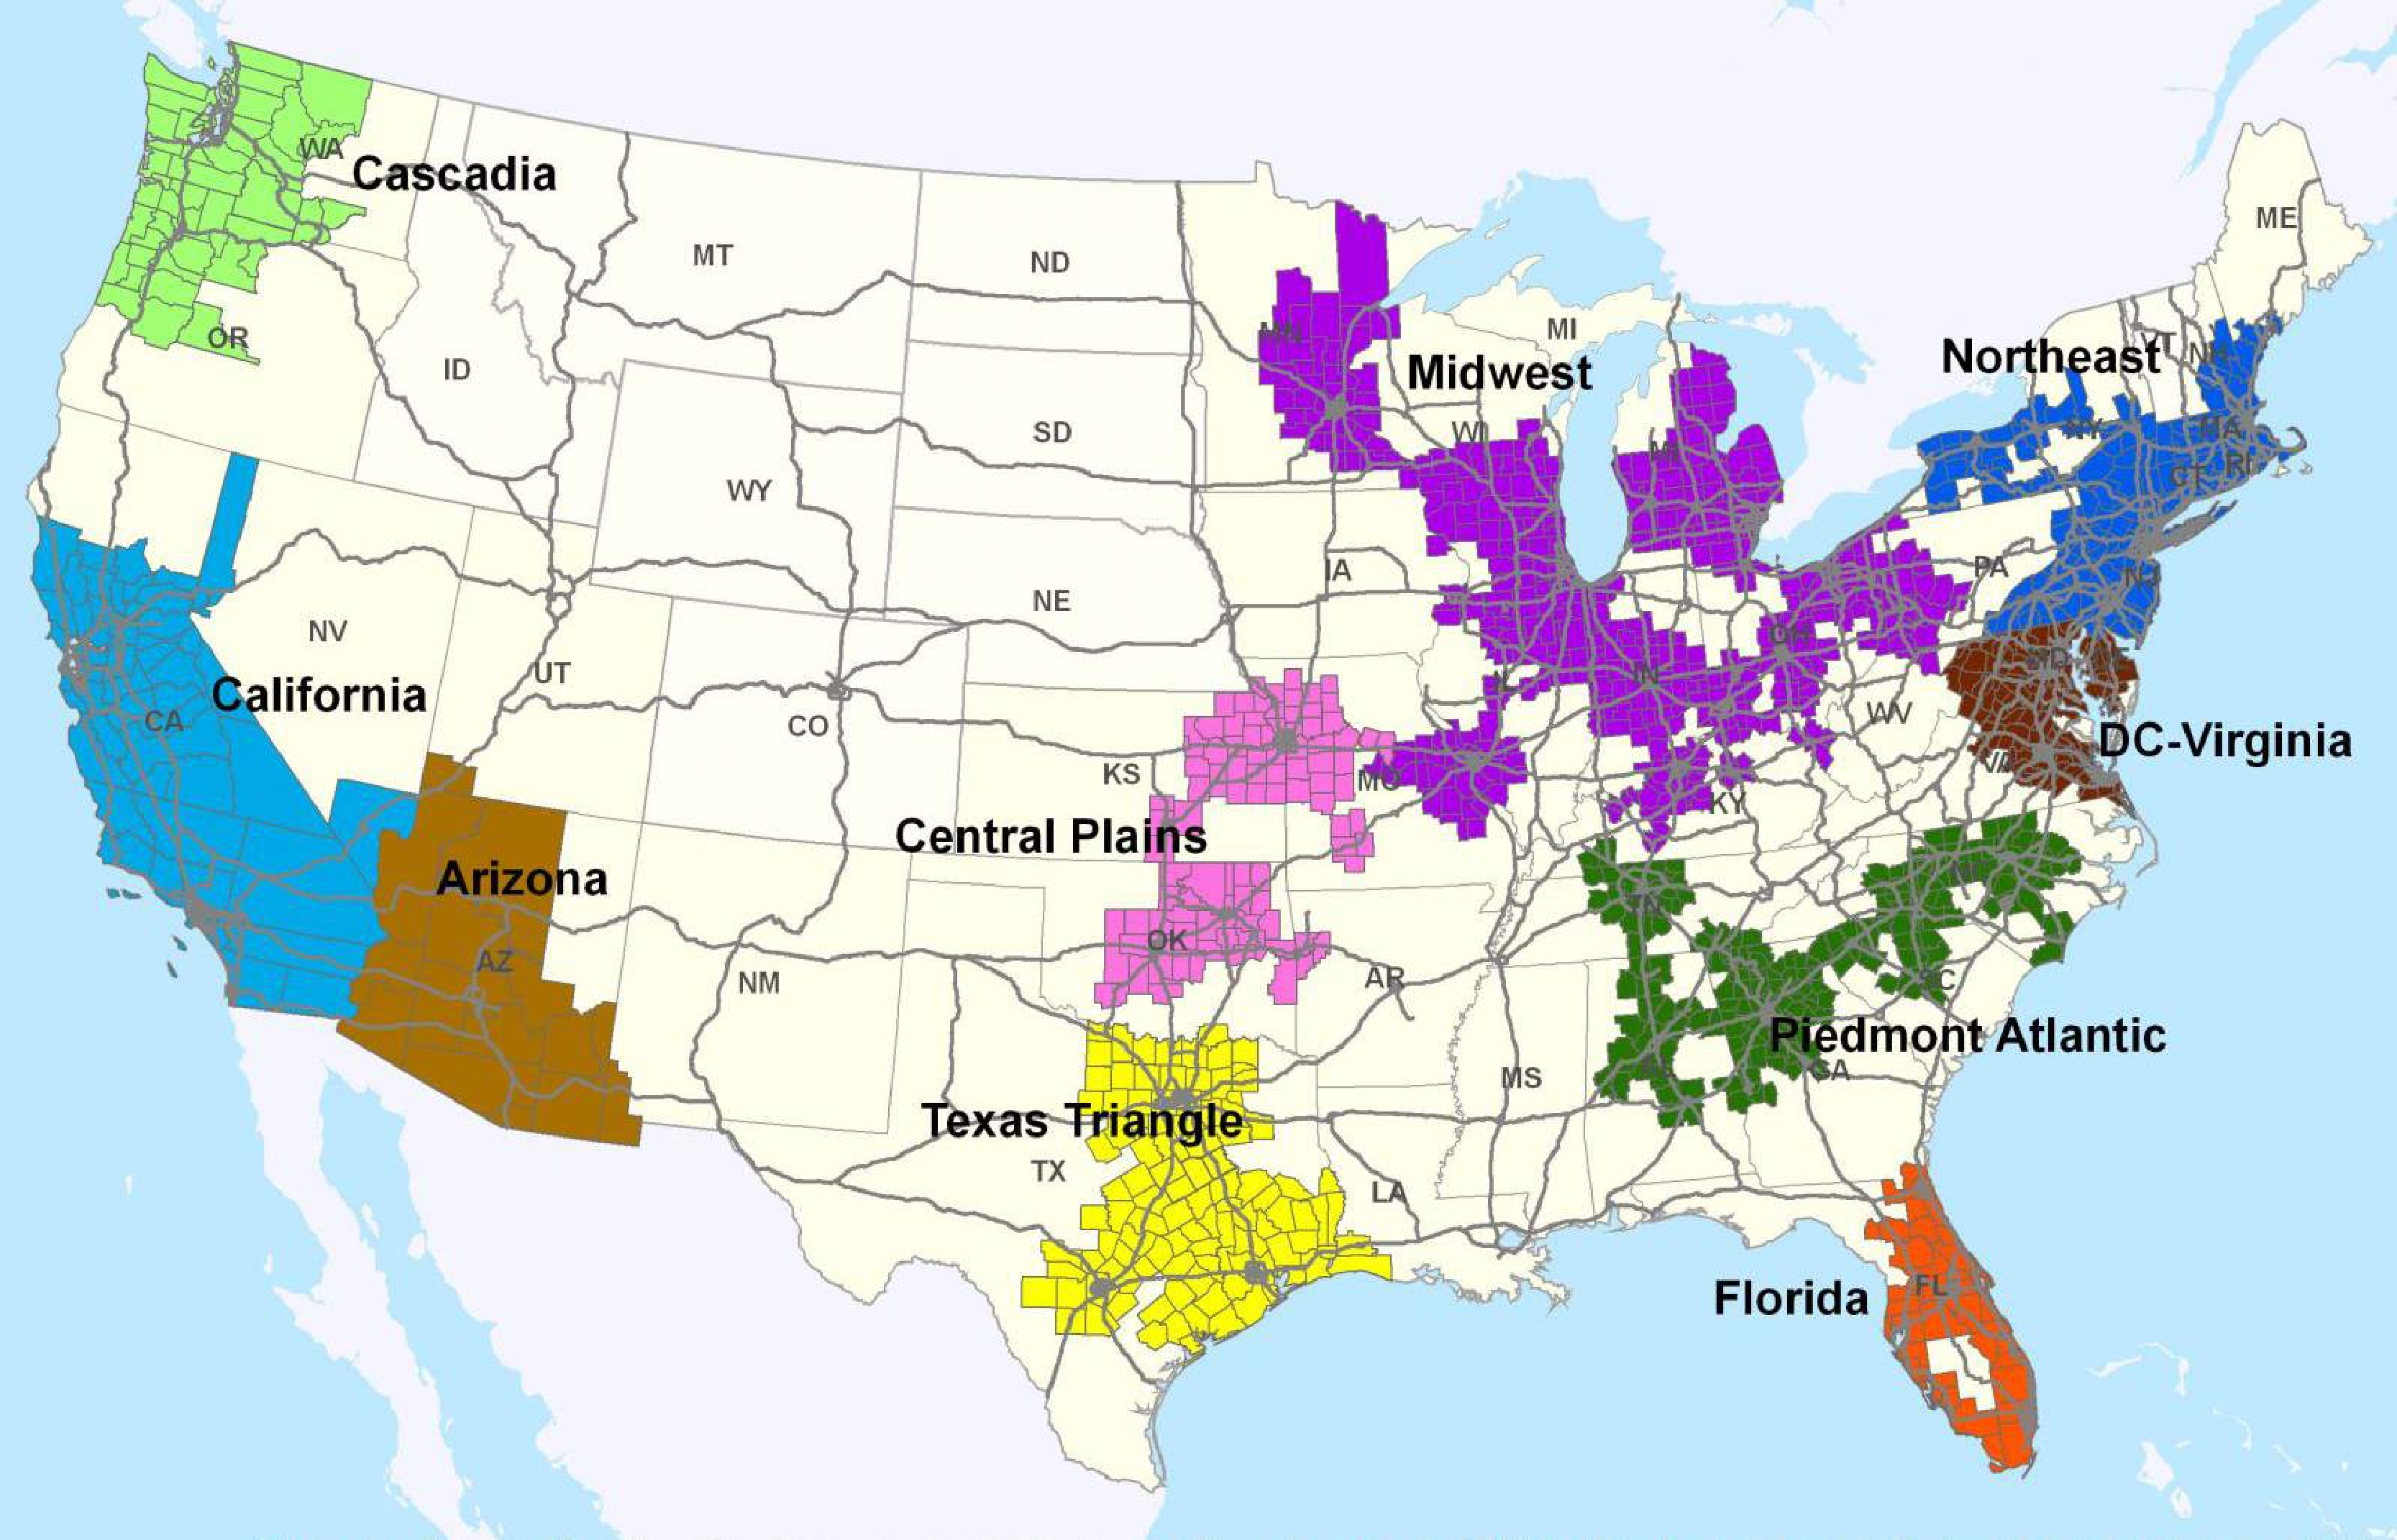
\includegraphics[width=6.5in]{graphics/02-megaregionsAccordingToRoss2009}
\caption[Delineation of ten megaregions in the U.S.]{Delineation of ten megaregions in the U.S. (Source: \cite{ross09b})}
\label{fig:ross-megaregions}
\end{figure}

In 2015, FHWA initiated an internal working group with representatives from several states and universities to foster megaregional analyses and activities. The five key interests of this working group are (in no particular order) freight, safety, economic vitality, infrastructure/transportation and environmental issues, all of which directly relate to transportation issues studied in megaregional models. The aim of the workgroup is to implement some form of an institution for each megaregion. However, the definition of institutions is left to the local jurisdictions to decide. Governance approaches for megaregions are not proposed by FHWA at this time. Nevertheless, FHWA helps to raise the awareness of the importance of megaregions and create synergies between agencies within megaregions.

FHWA also set up an online information system to support analyses on megaregions \citep{fhwa16a}. Under the category Megaregion Research, this website offers interactive maps that may be used to visualize 13 megaregions (as currently defined by FHWA) and compare them with the locations of MPO boundaries, highway networks, county population, GDP by MSA, truck volumes, among others.

For the time being, megaregions will be issue-based. Quasi-governmental structures to promote megaregions at large are not expected to be implemented soon. Problems that require joint action, such as highway corridors, rail corridors, protection of larger ecosystems or providing affordable housing, may lead to ad hoc creations of megaregional agencies with limited authority and under the tight control of state and/or metropolitan jurisdictions.

\subsection{Megaregional transportation models}\label{sec:megaregion-transport-models}

While there is a substantial body of literature on analyzing megaregions, little research has been conducted on modeling megaregions. The Chesapeake Bay Megaregional Model was implemented for the Washington, D.C. megaregion \citep{moeckel15b} as a FHWA demonstration project, and is described in more detail in \S\ref{sec:chesapeake-bay-megaregion-model} (page \pageref{sec:chesapeake-bay-megaregion-model}). As there are no institutionalized megaregional governance structures in place, there is no agency requesting continuous development of megaregional models. Existing models have been either issue-based (compare \S\ref{sec:hsr-megaregions}) or research-driven. Outside of federal initiatives, it is unlikely that megaregional models are built, maintained and applied.

While there are 29 operational statewide models plus five statewide models under development, only four megaregional models have been recently developed in the U.S. One is the Chesapeake Bay model described above. The remaining three are ad hoc models developed for specific purposes:
\begin{itemize}
\item \cite{zhang13} developed a model at the megaregional scale, but it is only intended for hurricane evacuation analysis of several southern states. The model focuses on the assignment step and models congestion depending on the areas needing evacuation if a hurricane is approaching.
\item A five-state model encompassing Texas and four neighboring states was built to evaluate interstate passenger rail corridors between them \citep{meyer15}. It provided analyses for the Southwest Multi-State Regional Plan, but does not appear to have been used otherwise.
\item Several statewide models are being fused to support analyses for the Appalachian Development Highway System Economic Analysis Study \citep{edrg16}. Details of the model are not yet available, but understood to represent synthesis and reconciliation of forecasts developed using several statewide models, and development of traffic assignment capabilities, rather than the development of a true megaregional model.
\end{itemize}

Outside the U.S., the Netherlands National Model System (NMS), often referred to by its Dutch name Landelijk Model Systeem (LMS), models travel demand for the entire Netherlands \citep{gunn94}. The SASI (Spatial and Socio-economic Impacts of Transport Investments and Transport System Improvements) models interactions of the economy with the transportation system for the entire European Union \citep{wegener08}. However, infrastructure benefits are only represented through accessibilities, which do not capture actual congestion on the transportation network.

Because of the limited number of existing megaregional models, this report clearly focuses on statewide modeling. Given the similarities in large-scale modeling, megaregional models are covered as a sibling of statewide modeling. With the recognition that the economic, social and environmental systems happen at the megaregional scale, unobstructed by municipal, county, MPO, or state boundaries, formal megaregional institutions with legislative power may be implemented in the future.

Many aspects of statewide modeling discussed in this report will apply to megaregional models as well. While one might argue that megaregions cover larger areas than states, the largest statewide models in operation (California and Texas) cover already a population and area larger than any megaregion in the U.S. The most important difference between megaregional and statewide modeling is that the former in most cases cover parts of several states, making it more challenging to reconcile input data and agree on issues that need to be addressed with the model.

\subsection{High-speed rail and megaregions}\label{sec:hsr-megaregions}

High-speed rail (HSR) has perhaps quietly become the most compelling case for megaregion modeling. New systems have been proposed in California, Florida, and Texas, whose statewide model coverage might be adequate for systems operating wholly within them. However, for other systems under consideration, the relevant markets cover multiple states, and their potential connections to existing intercity rail and air systems might involve even broader regions. Indeed, the potential for HSR seems to be one of the fundamental features used to define megaregions \citep{florida09, ross09b}.

All the known operational HSR models in North America are designed expressly for studying such systems. At most, they are one-way adaptations of existing statewide models, whose finished work does not appear to benefit the original model. In California, for example, the HSR Authority uses a modeling system that is separate from the California statewide model, as described in \S\ref{sec:california-hsr-model} (page \pageref{sec:california-hsr-model}). The former has taken advantage of data collected by the latter, but they remain otherwise separate works. In Texas, the statewide model was used to develop an inter-regional HSR model and forecasts. While data used to build the latter would certainly be useful in the evolution of the former, there are no known plans to integrate the two models. The first-generation Oregon statewide model was used to quickly examine the feasibility of HSR along the upper Pacific Coast, but the initiative never proceeded to formal study, which likely would have spawned the development of a custom model.

The development of separate HSR models seems to be more of tactical necessity than a long-term trend. In its defense, HSR forecasting requires more robust and sophisticated mode choice modeling than found in all but a handful of statewide models. The need to model the competitive response of air carriers, risk and uncertainty, and accuracy requirements exceed the capabilities of any known statewide or megaregion model. The Federal Railroad Administration also has unique analytical requirements at the preliminary, intermediate, and final stages that further influence the data and tools used to assess HSR ridership \citep{sdg11}.

Once built there would seem to be few impedances to using an HSR model as the first generation of a megaregion model. While it would need to be expanded to cover the many markets not addressed by HSR models, or at least not at the same level, many of the data used in their development would seem more broadly applicable. Due to the lack of megaregional governance structures discussed in \S\ref{sec:megaregion-transport-models}, however, such conversion from an HSR to a megaregion model has not occurred yet. Outside the specific interest (HSR), no agency has picked up such models for further analysis in different domains.

